\documentclass[a4paper,11pt]{article}
%\usepackage{epsf}
\usepackage{epsfig}
\usepackage{graphics}
%define the title
\title{Quiz for section 4.4, 4.8, 4.9}
\begin{document}
%generates the title
\maketitle
\paragraph{Problem 1}
The Cissoid of Diocles is the solution set of

\begin{equation}
x^3+xy-2y^2=0
\end{equation}

It looks like:

\begin{figure}[h]
\begin{center}
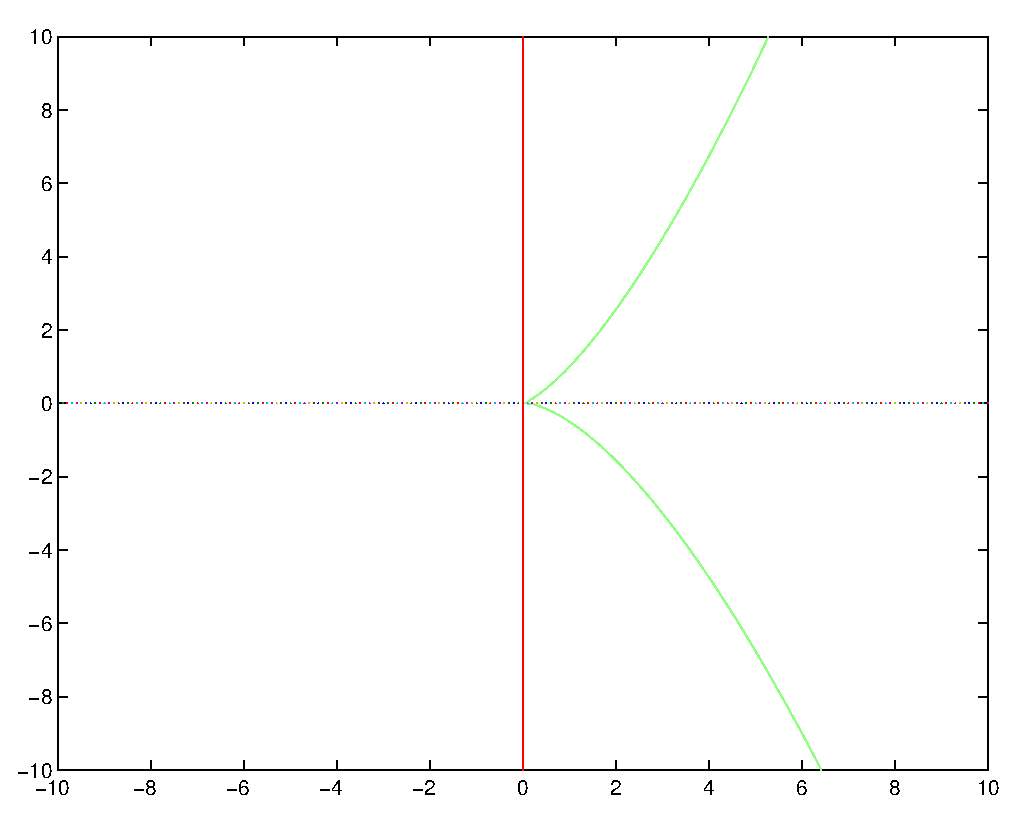
\epsfig{file=cissoid.eps, height=2.25in}
%\epsfxsize=2in {\epsfbox{fig.eps}}
%\caption{\small \sl Cissoid of Diocles.}
%\label{fig:Stupendous}
\end{center}
\end{figure}

Find the equation for the tangent line to the Cissoid at the point (1,1).
\vspace{3in}

\paragraph{Problem 2}
Using differentials, estimate cos($28\,^{\circ}$).
\vspace{1in}

\paragraph{Problem 3}
A man in a hot-air balloon is ascending at a rate of 10ft/sec.  How fast is
the distance from the horizon increasing when the balloon is 1,000 feet
high?  Assume the earth's radius is 4000 mile.
\begin{figure}[h]
\begin{flushright}
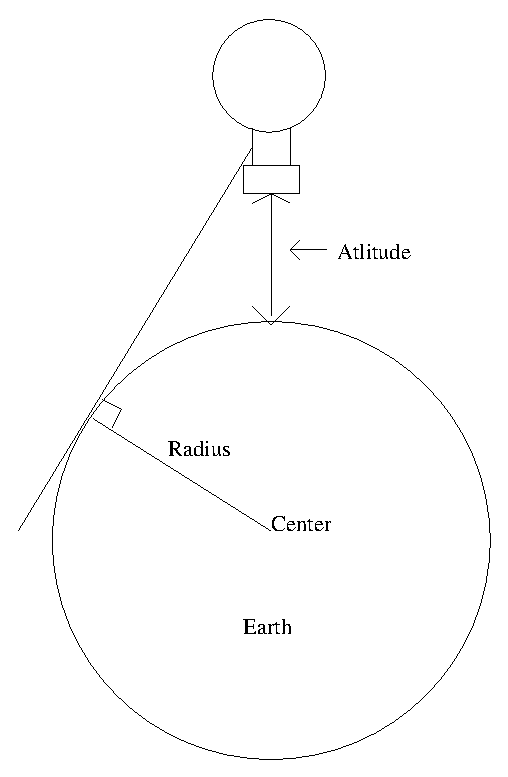
\epsfig{file=hotairballoon.eps, height=3in}
\end{flushright}
\end{figure}
%\vspace{3in}

\paragraph{Problem 4}
Calculate the differentials:

\subparagraph{(a)}
$d\left(\sqrt{1-x^2}\right)$
\vspace{0.4in}

\subparagraph{(b)}
$d\left(\frac{1}{sin^3(x)}\right)$
\vspace{0.4in}

\subparagraph{(c)}
$d\left(\frac{x+1}{x-1}\right)$
\vspace{0.4in}

\end{document}
